% Created 2022-07-03 Sun 02:38
% Intended LaTeX compiler: pdflatex
\documentclass[titlepage,a4paper]{article}
\usepackage[utf8]{inputenc}
\usepackage[T1]{fontenc}
\usepackage{graphicx}
\usepackage{longtable}
\usepackage{wrapfig}
\usepackage{rotating}
\usepackage[normalem]{ulem}
\usepackage{amsmath}
\usepackage{amssymb}
\usepackage{capt-of}
\usepackage{hyperref}
\usepackage{minted}
\hypersetup{colorlinks=true,linkcolor=black,urlcolor=blue,bookmarksopen=true}
\usepackage{a4wide}
\usepackage{bookmark}
\usepackage{fancyhdr}
\usepackage[spanish]{babel}
\usepackage[utf8]{inputenc}
\usepackage[T1]{fontenc}
\usepackage{graphicx}
\usepackage{float}
\usepackage{minted}
\usepackage{svg}
\pagestyle{fancy}
\fancyhf{}
\fancyhead[L]{TP3 - Grupo 1}
\fancyhead[R]{Teoria de Algoritmos I - FIUBA}
\renewcommand{\headrulewidth}{0.4pt}
\fancyfoot[C]{\thepage}
\renewcommand{\footrulewidth}{0.4pt}
\usemintedstyle{stata-light}
\newminted{c}{bgcolor={rgb}{0.95,0.95,0.95}}
\usepackage{color}
\usepackage[utf8]{inputenc}
\usepackage{fancyvrb}
\fvset{framesep=1mm,fontfamily=courier,fontsize=\scriptsize,numbers=left,framerule=.3mm,numbersep=1mm,commandchars=\\\{\}}
\usepackage[nottoc]{tocbibind}
\date{\today}
\title{}
\hypersetup{
 pdfauthor={},
 pdftitle={},
 pdfkeywords={},
 pdfsubject={},
 pdfcreator={Emacs 29.0.50 (Org mode 9.5.4)}, 
 pdflang={Spanish}}
\begin{document}

\begin{titlepage}
    \hfill
\includegraphics[width=6cm]{assets/logofiuba.jpg}
    \centering
    \vfill
    \Huge \textbf{Trabajo Práctico 2 — GPS Challenge}
    \vskip2cm
    \Large [75.07/95.02] Algoritmos y Programación III \\
    Primer cuatrimestre de 2022\\
    \vfill
    \begin{tabular}{ | l | l | l | }
      \hline
      Alumno & Padron & Email \\ \hline
      CASTILLO, Carlos & 108535 & ccastillo@fi.uba.ar \\ \hline
      DEALBERA, Pablo Andres & 106585 & pdealbera@fi.uba.ar \\ \hline
      DUARTE, Luciano & 105604 & lduarte@fi.uba.ar \\ \hline
      RECCHIA, Ramiro & 99289 & rrecchia@fi.uba.ar \\ \hline
    \end{tabular}
    \vfill
    \begin{tabular}{ | l | l | }
      \hline
      Corrector & Email \\ \hline
      GOMEZ, Joaquin & gjoaquin@fi.uba.ar \\ \hline
      VALDEZ, Santiago & vsantiago@fi.uba.ar \\ \hline
    \end{tabular}
    \vfill
\end{titlepage}
\tableofcontents
\newpage
\definecolor{bg}{rgb}{0.95,0.95,0.95}

\section{Supuestos}
\label{sec:org47d20ed}

\section{Diagramas de clases}
\label{sec:org1f4f733}
\subsection{Vehiculo}
\label{sec:org7c37a4f}

\begin{center}
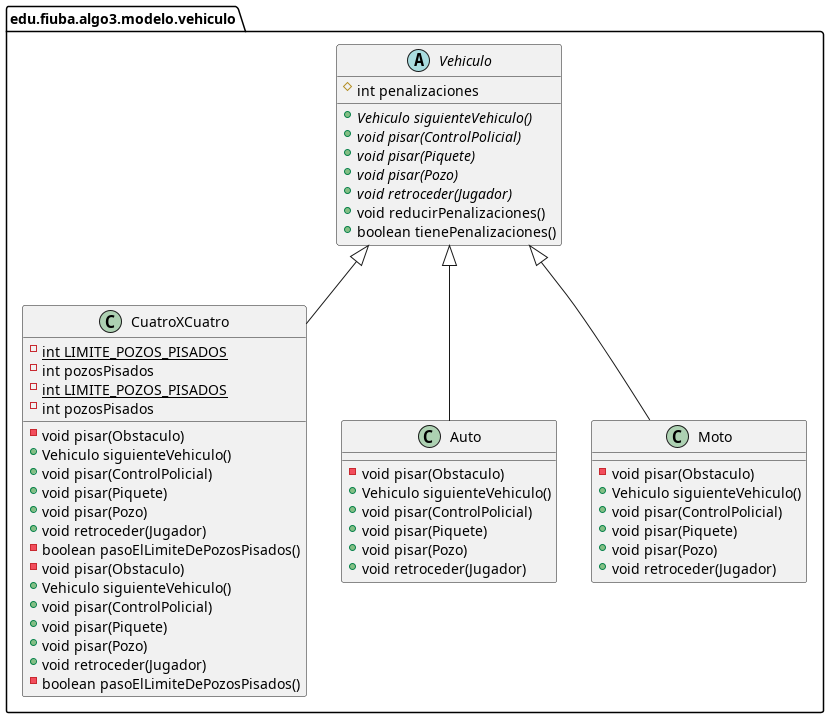
\includegraphics[width=.9\linewidth]{./diagramas/clases-vehiculo.png}
\end{center}

\subsection{Sorpresas}
\label{sec:org7c29ca0}

\begin{center}
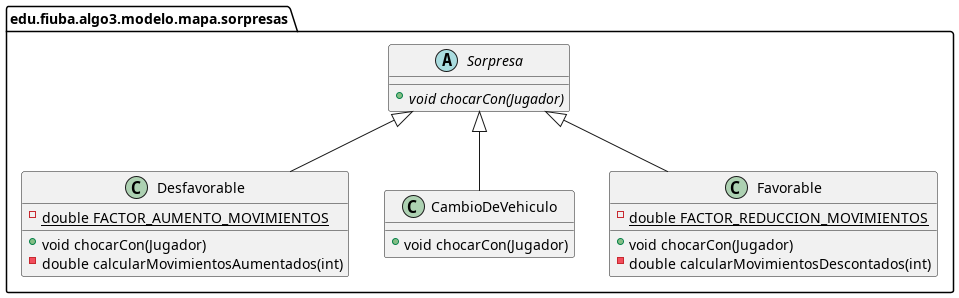
\includegraphics[width=.9\linewidth]{./diagramas/clases-sorpresas.png}
\end{center}

\subsection{Obstaculos}
\label{sec:orgd6f2170}

\begin{center}
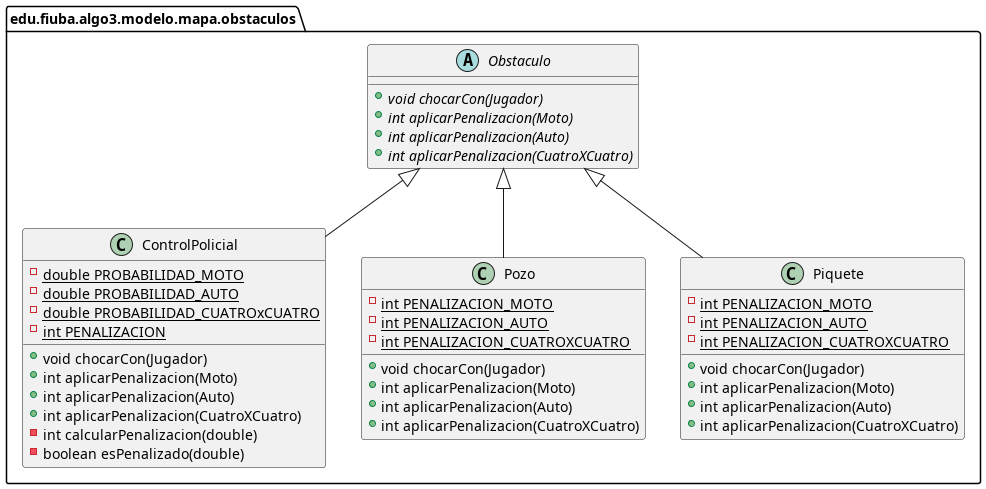
\includegraphics[width=.9\linewidth]{./diagramas/clases-obstaculos.png}
\end{center}

\subsection{Mapa}
\label{sec:orgbf8a59a}

\begin{center}
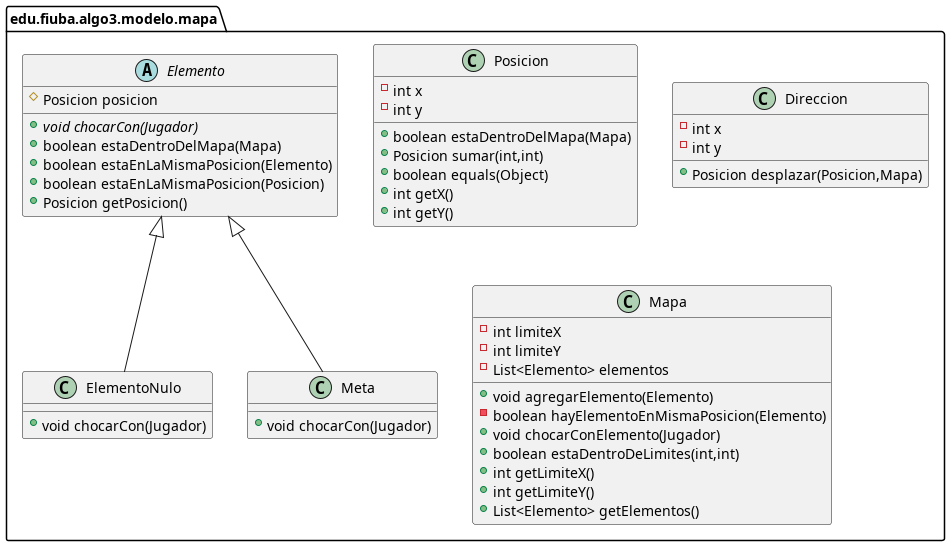
\includegraphics[width=.9\linewidth]{./diagramas/clases-mapa.png}
\end{center}

\subsection{ModeloJuego}
\label{sec:orgd94c462}

\begin{center}
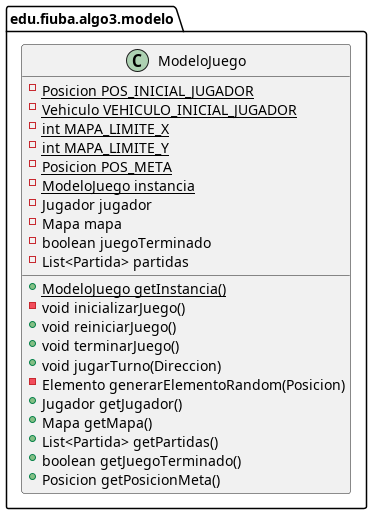
\includegraphics[width=.9\linewidth]{./diagramas/clases-modelojuego.png}
\end{center}


\section{Diagrama de paquetes}
\label{sec:org0f3b886}
\begin{center}
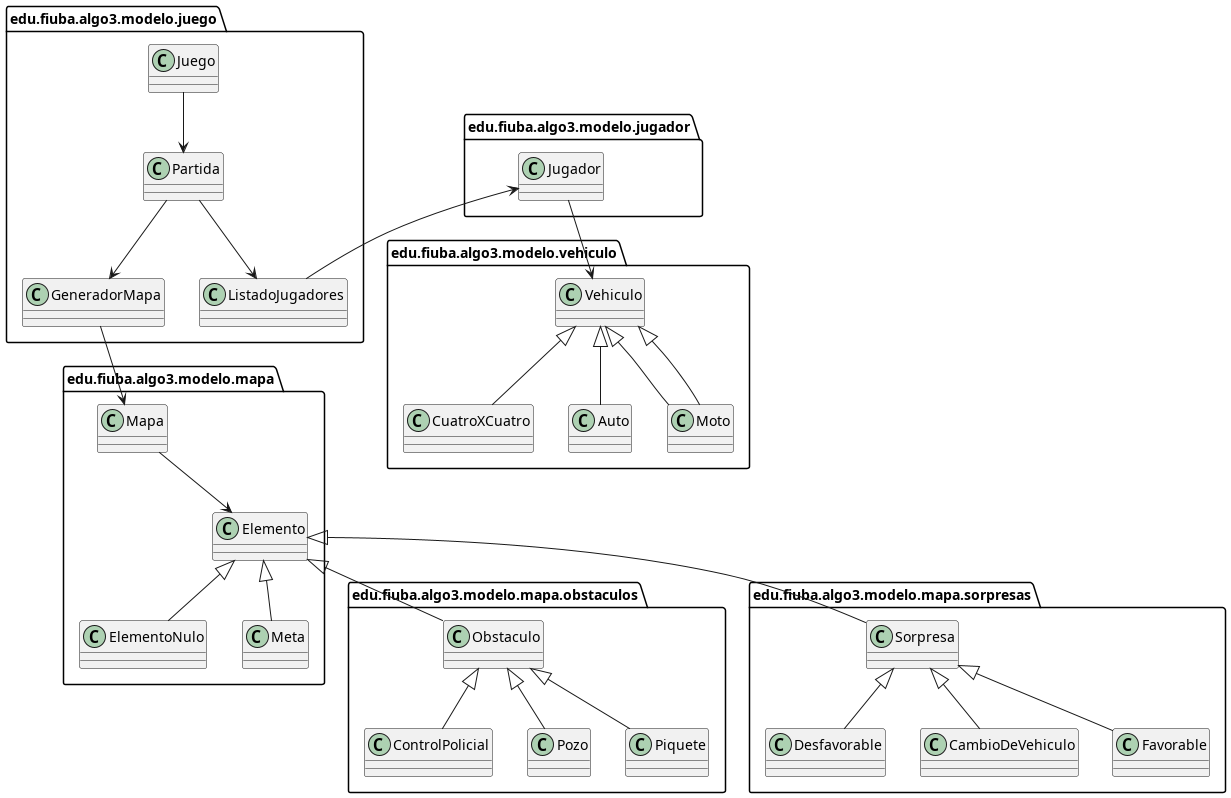
\includegraphics[width=.9\linewidth]{./diagramas/paquetes.png}
\end{center}

\section{Diagramas de secuencia}
\label{sec:orgaa75bd2}
\subsection{Interaccion Jugador - Sorpresa Cambio de Vehiculo}
\label{sec:org1a2737b}

\begin{center}
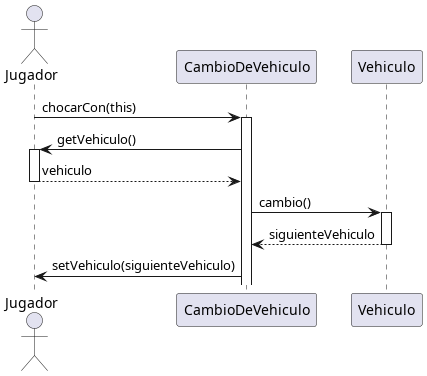
\includegraphics[width=.9\linewidth]{./diagramas/jugadorAvanzaYSeEncuentraConUnaSorpresaCambioDeVehiculo.png}
\end{center}

\subsection{Interaccion Jugador - Sorpresa Favorable}
\label{sec:orgb06de5b}

\begin{center}
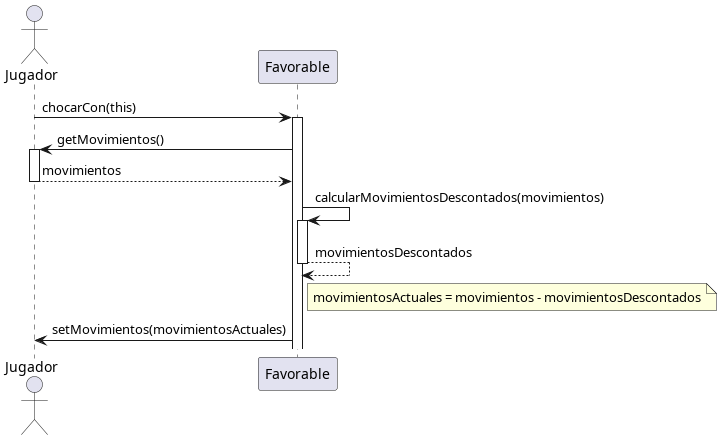
\includegraphics[width=.9\linewidth]{./diagramas/jugadorAvanzaYSeEncuentraConUnaSorpresaFavorable.png}
\end{center}

\subsection{Interaccion Jugador - Elemento}
\label{sec:orgefc330c}

\begin{center}
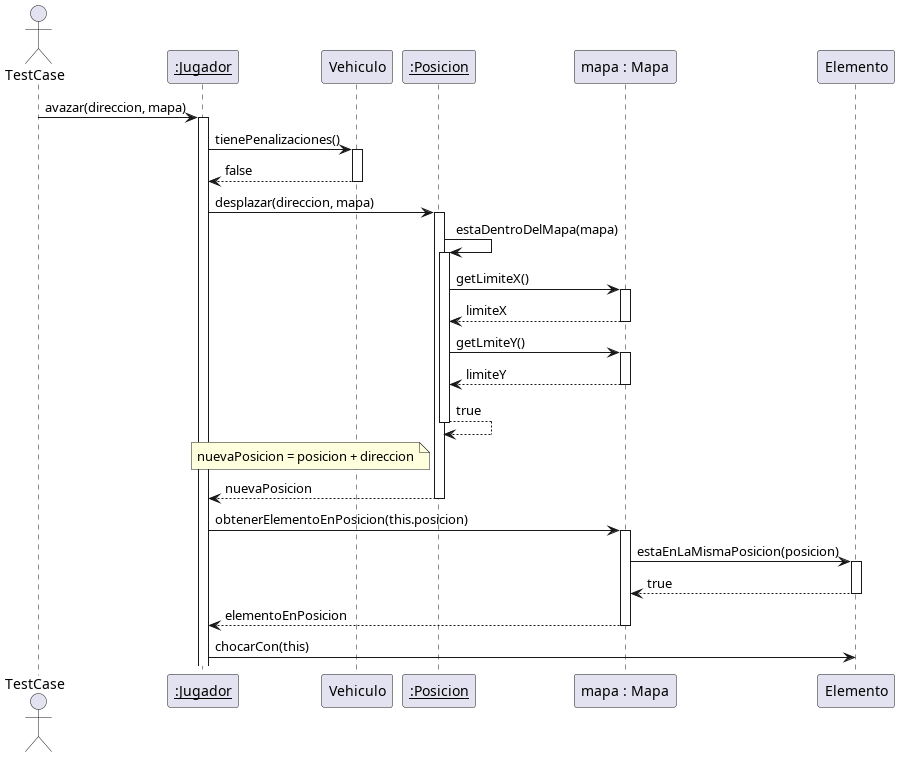
\includegraphics[width=.9\linewidth]{./diagramas/jugadorAvanzaYSeEncuentraConUnElemento.png}
\end{center}

\subsection{Jugador avanza y se encuentra con un Elemento}
\label{sec:orgd0a9b83}

\begin{center}
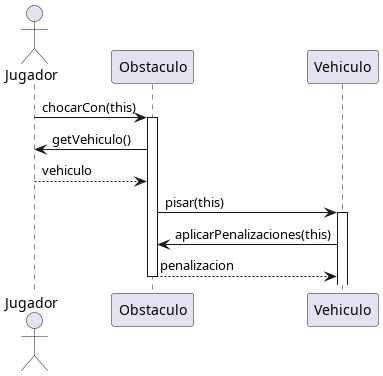
\includegraphics[width=.9\linewidth]{./diagramas/jugadorAvanzaYSeEncuentraConUnObstaculo.png}
\end{center}

\section{Diagramas de estado}
\label{sec:org8480b0f}

\section{Detalles de implementación}
\label{sec:org59ef13e}
\subsection{Vehiculo}
\label{sec:orgb5896ff}

En principio tenes una clase abstracta llamada \emph{Vehiculo} y usamos herencia para
abstraer comportamiento comun entre su tres clases hijas: Moto, Auto y CuatroXCuatro.

\subsection{Elemento}
\label{sec:org93decb1}

Es una clase abstracta de la cual heredan dos clases:

\begin{itemize}
\item Obstaculo
\begin{itemize}
\item Pozo, Piquete y Control Policial.
\end{itemize}
\item Sorpresa
\begin{itemize}
\item Favorable y Cambio de Vehiculo
\end{itemize}
\item Meta
\end{itemize}

Utilizamos esta clase para definir compotamientos que los distintos
Elementos tienen en comun, como por ejemplo que pueden \texttt{chocaCon} un
jugador, y algunas funciones de ayuda para saber si el elemento esta
adentro del mapa, si esta en la misma posicion que otro elemento o una
posicion arbitraria, etc.

\subsection{Interaccion Vehiculo-Obstaculo}
\label{sec:org8f3d271}

Para la interaccion Vehiculo-Obstaculo decidimos usar el patron \emph{Double
Dispatch} de forma ya que tenemos una interaccion de muchos a muchos entre los
hijos de ambas clases abstractas:

\begin{center}
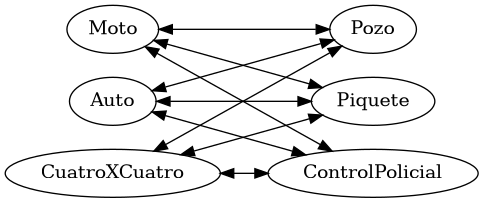
\includegraphics[width=.9\linewidth]{diagramas/interaccionVehiculoObstaculo.png}
\end{center}

Ademas de esto teniamos la necesidad de modelar implementaciones especificas
como el caso de CuatroXCuatro-Pozo donde la CuatroXCuatro debe pisar tres pozos
para recibir una penalizacion, cosa que no sucede en ninguna de las otras interacciones.

Para esto los Vehiculos tienen firmas segun cada implementacion de Obstaculo.
Y cada implementacion de Obstaculo tiene firmas para cada Vehiculo.

\section{Excepciones}
\label{sec:org12b8a92}
\end{document}